\chapter{Results}
\label{chap:Results}

\section{Limit Setting}
As no significant signal is observed, limit for the $\mathcal{B}(\Bmumumu)$ is set. This is achieved by using the $CL_{s}$ method described in~\autoref{sensitivity} and the $CL_{s}$ $p$ values are shown in ~\autoref{fig:limitset} together with both expected and observed curves. In this limit setting procedure where simultaneous fits are used, the systematic uncertainties mostly affect the efficiency ratios. In order to incorporate the systematics uncertainties in the limit setting they are added as 1D Gaussian constraints on the relevant efficiency ratios when calculating limit. They are assumed to be 100\% correlated between the bins of fractional corrected mass error but uncorrelated between the different effects.
 This gives following limits summarised in~\autoref{tab:limits}, setting the limit $\mathcal{B}(\Bmumumu) < 1.1(1.4)\times 10^{-8}$ at $90\%(95\%)$ confidence level. As it can be seen, observed limit is better than expected limit resulting in a downward fluctuation of around 1$\sigma$ compared to the expected sensitivity.

\begin{figure}[H]
\begin{center}
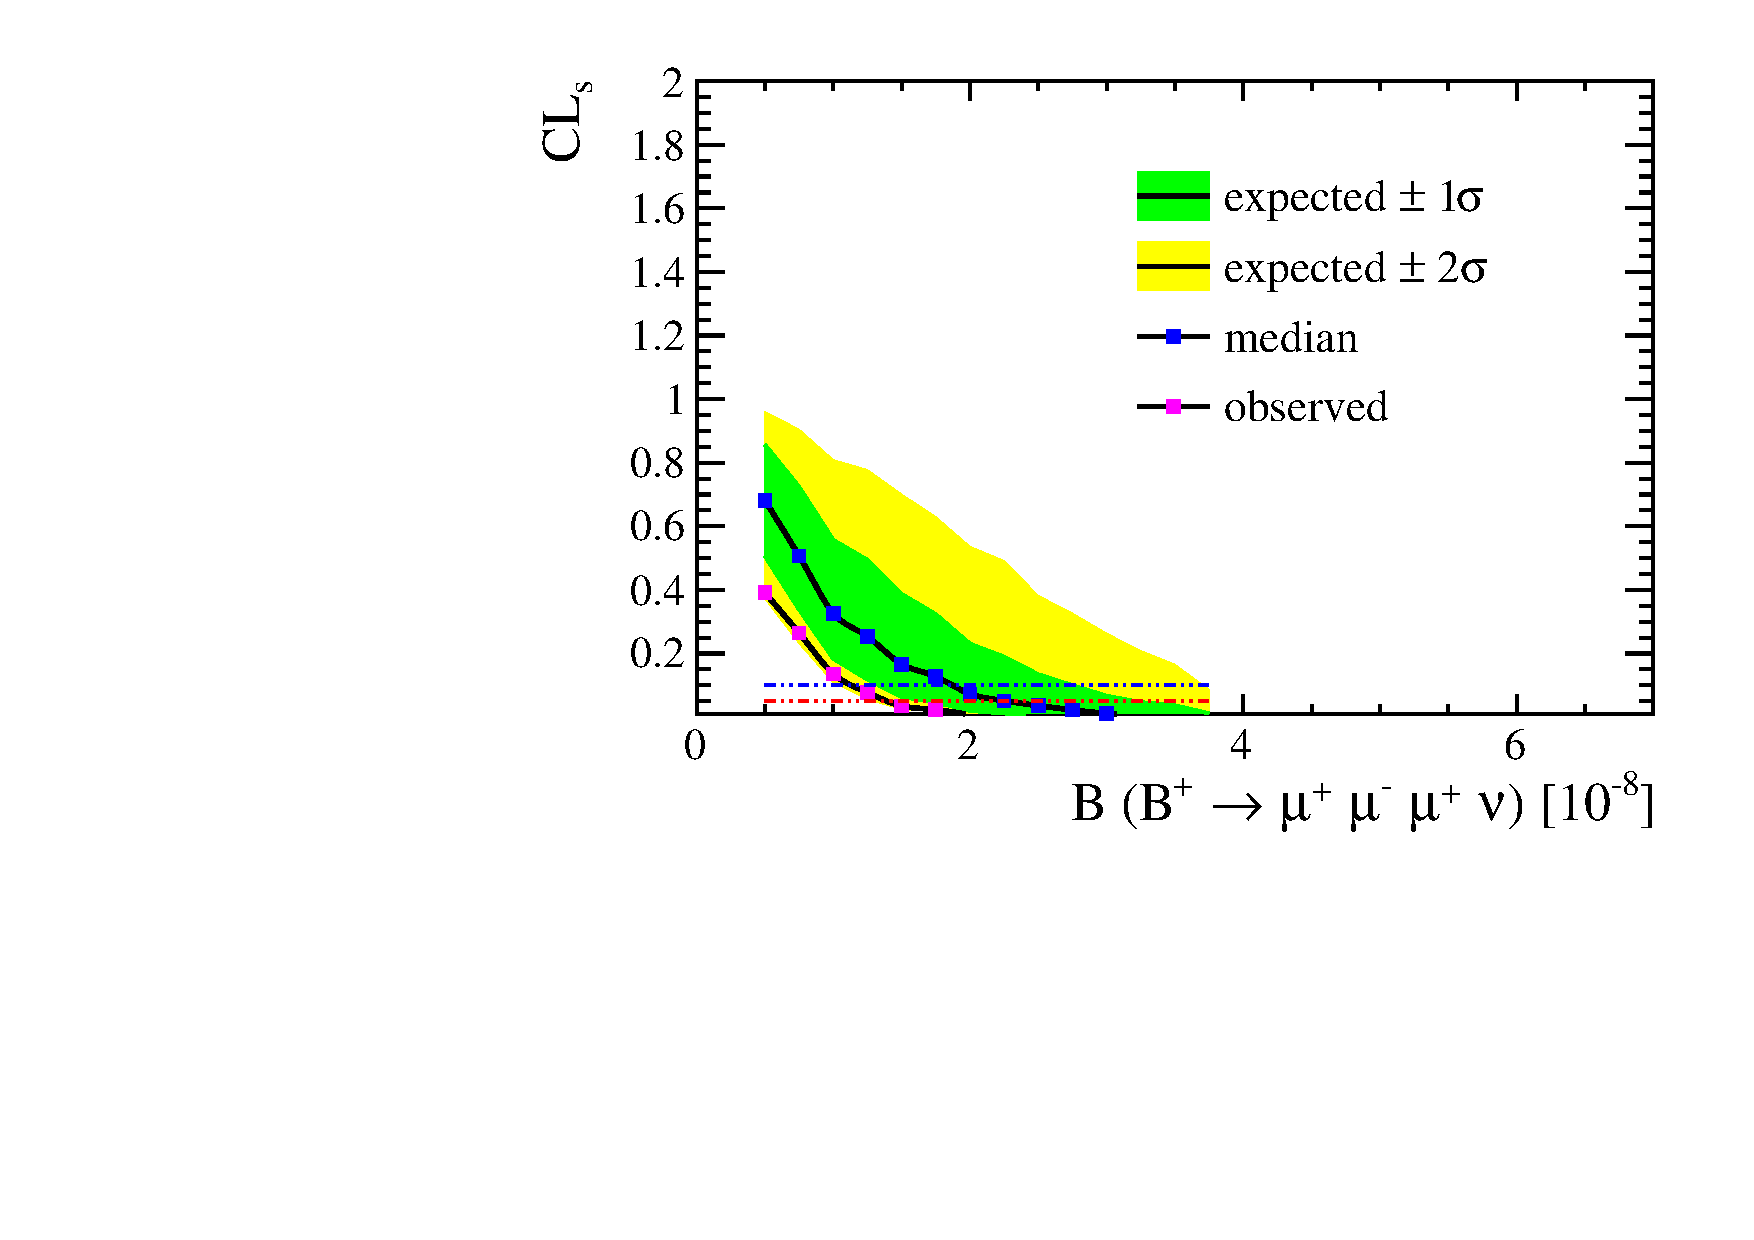
\includegraphics[width=0.5\linewidth]{./results/ClsExclusion_new_picked_final.pdf}\put(-30,100){(a)}%
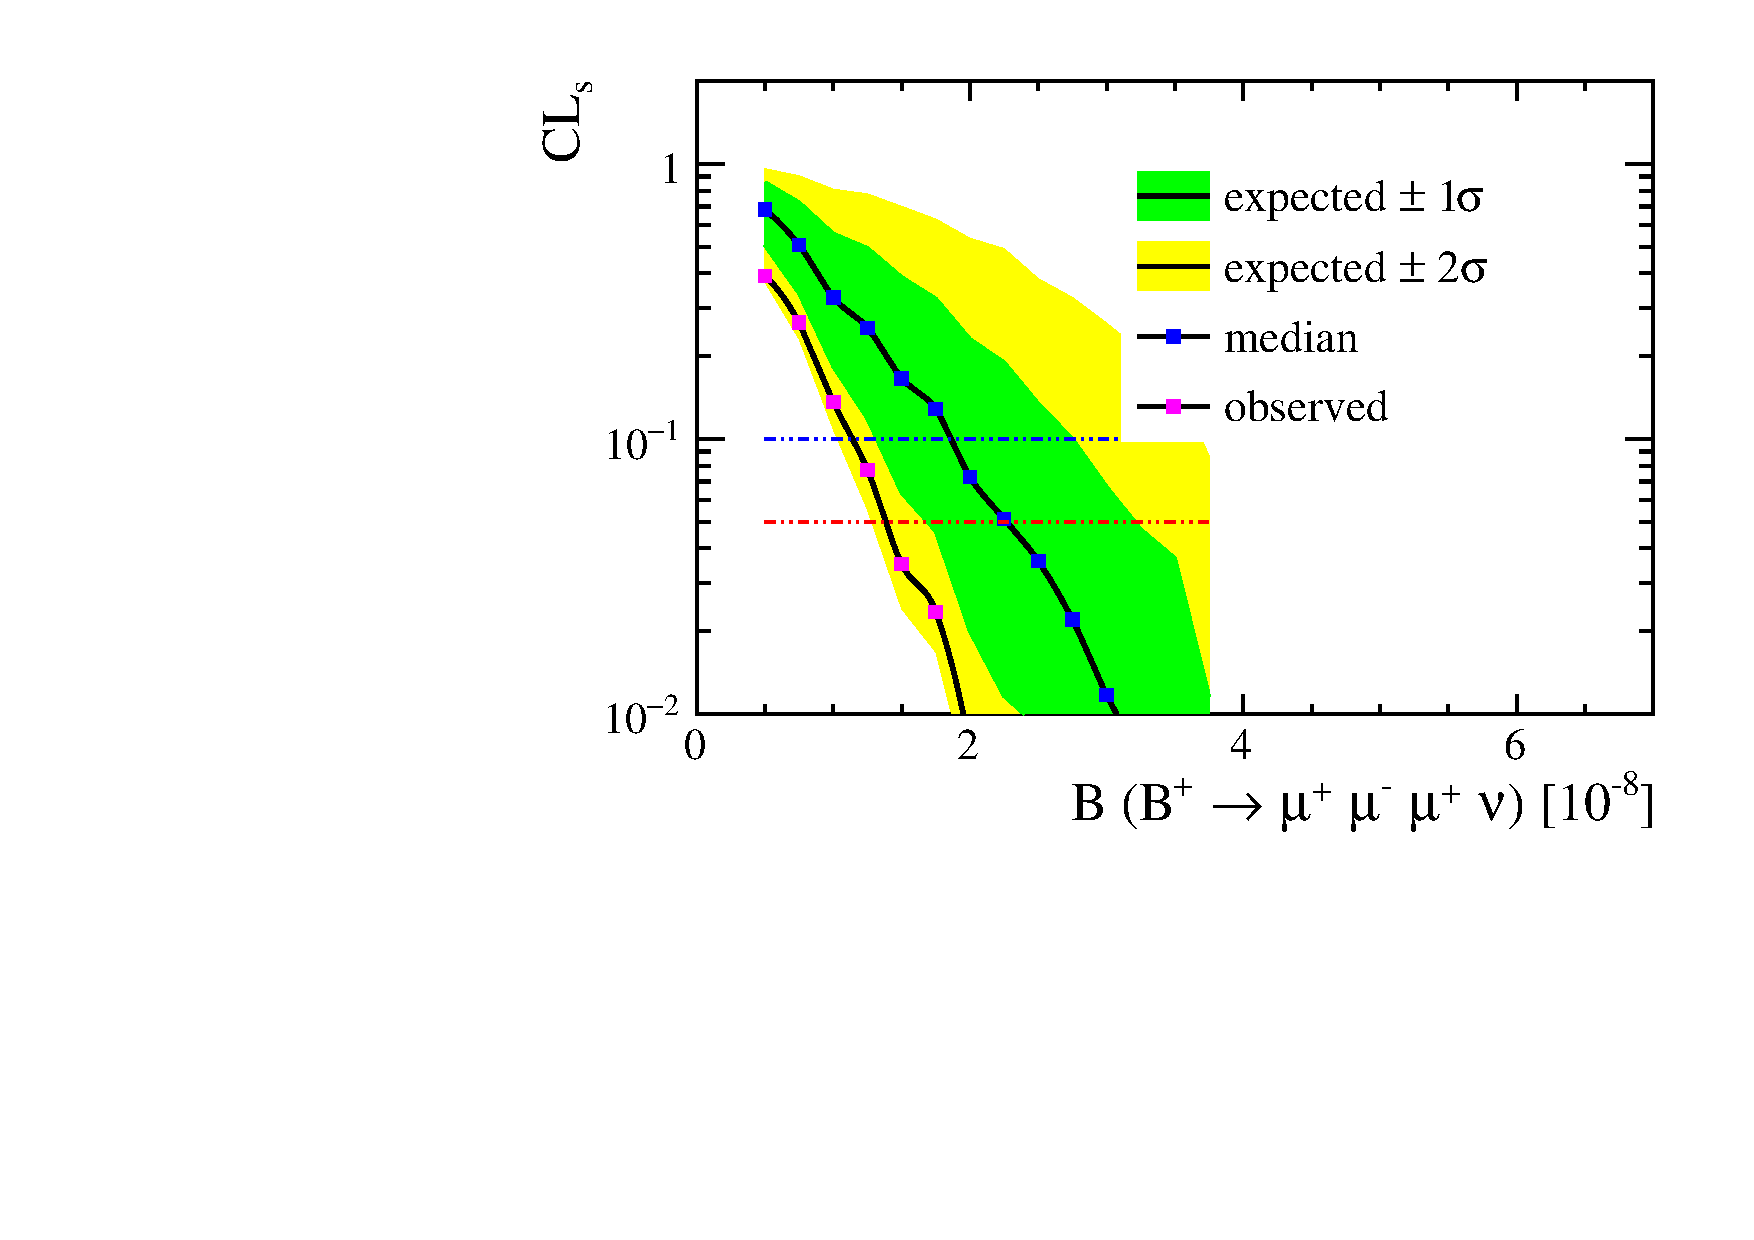
\includegraphics[width=0.5\linewidth]{./results/ClsExclusion_new_Log_picked.pdf}\put(-30,100){(b)}
\caption{Expected and observed 90\% (blue horizontal line) 95\% (red horizontal line) CL exclusion limits for full Run 1 and 2016 simultaneous data fit accounting for all systematics with (a) normal and (b) logarithmic y-axis.}% (c) Not simultaneous (d) simultaneous expected exclusion limits on the branching fraction to full Run 1 + 2016 dataset. As expected simultaneous fit to all data yields the best sensitivity with 2.5$\times$10$^{-8}$ at 95\% CL.}
\label{fig:limitset}
\end{center}
\end{figure}


\begin{table}[H]
\centering
%\small
\begin{tabular}{ l  l  l  }
\toprule
Expected/Observed & CI & Value  \\ \hline
Expected & $90\%$ CL & $ 1.9\times 10^{-8}$ \\
Observed & $90\%$ CL & $ 1.1\times 10^{-8}$ \\
Expected & $95\%$ CL & $ 2.3\times 10^{-8}$ \\
Observed & $95\%$ CL & $ 1.4\times 10^{-8}$ \\
\bottomrule
\end{tabular}
\caption{Resulting exclusion limits with simultaneous fit.}
\label{tab:limits}
\end{table}

\section{Conclusion}
In conclusion most of this thesis was dedicated to the search of the \Bmumumu.
This search was perfomed using 4.7\invfb of proton-proton collision data collected by the \gls{LHCb} experiment. No significant signal was observed for \Bmumumu and an upper limit of $< 1.4\times 10^{-8}$ at 95\%~confidence level was set for the branching fraction, where the minimum of the two $\mumu$ mass combinations is below $980$\mevcc. This limit disagrees with a recent theoretical calculation based on the vector dominance model~\cite{Danilina:2018uzr}, where the $\mathcal{B}(\Bmumumu)=1.3\times 10^{-8}$. In order to visualize the fit with this branching fraction hypothesis, the fit is plotted in~\autoref{fig:signalfit}. It can be seen that this signal would have been clearly visible if it was there. Under the assumption that the decay is dominated by intermediate vector mesons, the limit for the full kinematic region stays the same.


\begin{figure}[t]
  \centering
  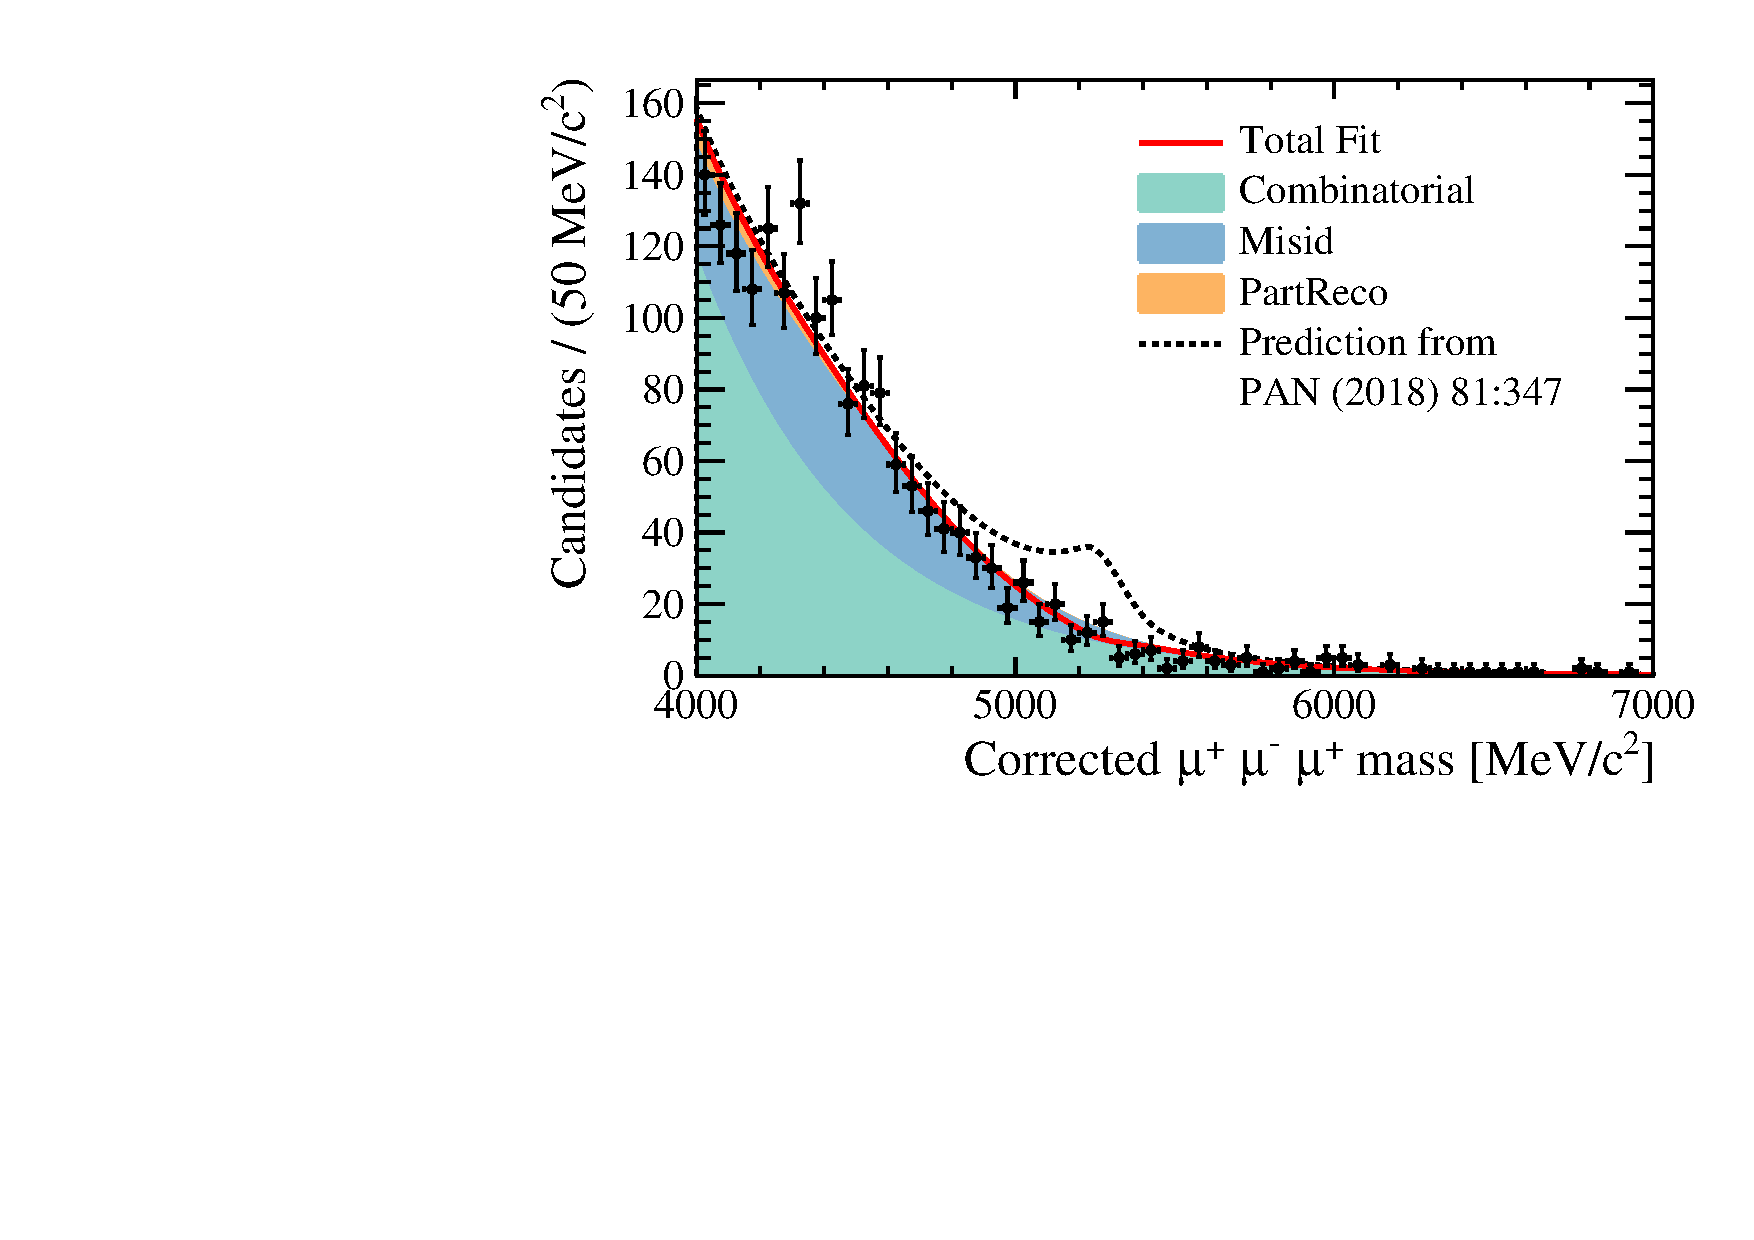
\includegraphics[width=0.80\linewidth]{results/fit.pdf}
  \caption{Corrected mass distribution of all selected \Bmumumu
    candidates with the fit overlaid. Samples with low and high
    corrected mass uncertainty are fitted as individual samples but
    are merged in the figure. As the signal yield is negative the total fit
    in red shows a downward fluctuation. The dashed line represents the fit
    result if the signal had the branching fraction predicted in~\cite{Danilina:2018uzr}.}
  \label{fig:signalfit}
\end{figure}


This thesis also presented \gls{PID} work that concentrated on the correlation induced by having more than one muon in a final state.


\section{Outlook}
Despite the fact that no signal was observed, a stringent limit on the $\mathcal{B}(\Bmumumu)$ was set with direct impact on prediction given by ~\cite{Danilina:2018uzr}. As mentioned in~\autoref{mydecay}, the naive estimate of $\mathcal{B}(\Bmumumu)=1.0\times 10^{-8}$ is therefore not too far from the set limit. At the moment of the writing of this thesis \gls{LHCb} collected 8\invfb of data, which means that the dataset for the analysis doubled. So assuming that the dataset doubles with the same ratio between the background and signal the limit would improve by a factor of $1/\sqrt{2}$, which would reach the the naive branching fraction estimate. 


